\section{Results and Tests}
To test the energy consumption of the game, the eAProfiler tool was used. First,
as can be seen in figure \ref{fig:nosleep}, a version of the game where the game loop
is running non stop was tested. The interesting thing to see is the comparison
to figure \ref{fig:sleep}, where the device goes to sleep after each iteration
of the game loop, and only wakes up when it is time to draw a new frame.

\begin{figure}[H]
\centering
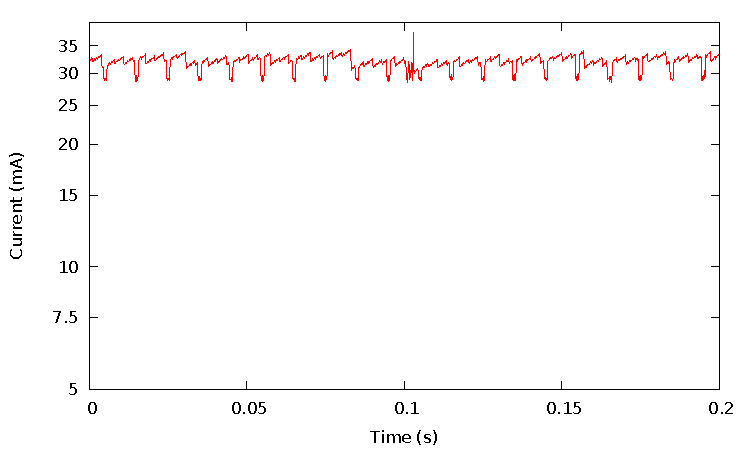
\includegraphics[width=0.7\textwidth]{figures/nosleep.pdf}
\caption{Graph of non sleeping code}
\label{fig:nosleep}
\end{figure}

\begin{figure}[H]
\centering
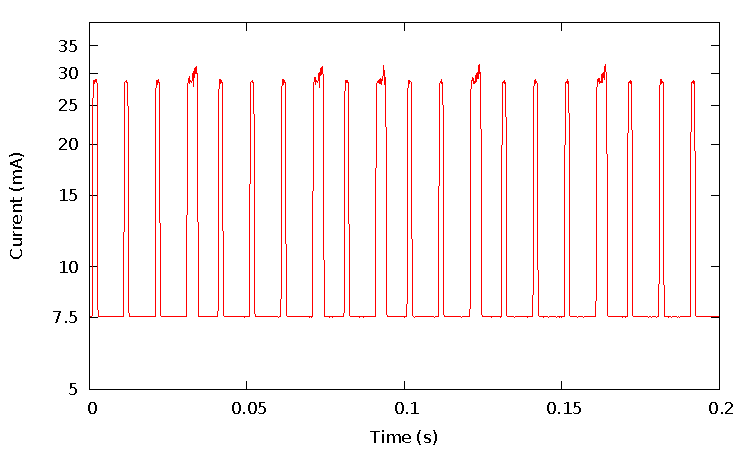
\includegraphics[width=0.7\textwidth]{figures/sleep.pdf}
\caption{Graph of sleeping code}
\label{fig:sleep}
\end{figure}

The power usage of the different implementations are nearly identical in the
peaks, but as shown in figure \ref{fig:sleep}, the game saves a lot of energy by
going into a low powered state when not having to do anything.

% Sleeping: 7.59mA
% Awake: 29.01mA
% Total: 11.95mA
% Averaged over 10 seconds
